\chapter{Technical Design Development}

\section{Organisational Breakdown Structure}
In order to optimise technical development, the team has identified critical, non-technical, roles and tasks, which were then distributed amongst its members. The roles identified are the following:


\begin{figure}[h]
    \centering
    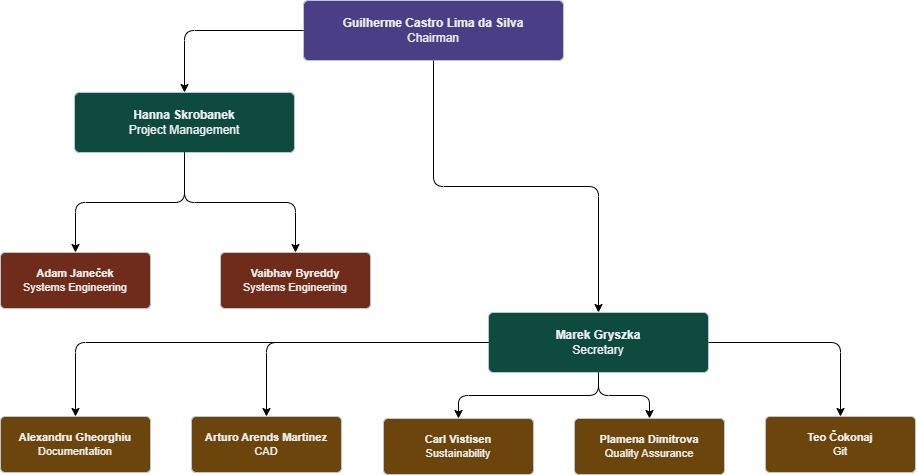
\includegraphics[width=\linewidth]{figures/Group 28 Organigram.jpg}
    \caption{Organigram detailing the organisational structure of Group 28}
    \label{fig:organogram}
\end{figure}

\section{Team technical roles}
According to the project guide \autoref{}, where percentages of relevant technical expertise required for the project are stated, the team divided into several sub-groups based on the technical expertise of its members. The technical expertise groups were labelled as \textbf{AERO}, representing aerodynamics, performance and propulsion, \textbf{ASM}, representing materials and manufacturing, and \textbf{CONTROL}, representing control and stability, systems engineering and operations. Besides the roles assigned in \autoref{fig:organogram}. The preferences of each team member are presented in \autoref{}.

\begin{table}[H]
    \centering
    \begin{tabular}{|c|c|}
         &  \\
         \hline
         &  \\
         \hline
    \end{tabular}
    \caption{Caption}
    \label{tab:placeholder}
\end{table}